\documentclass[UTF8,a4paper,12pt]{ctexart}
\usepackage[margin=2.45cm]{geometry}
\usepackage{graphicx}
\usepackage{booktabs}
\usepackage{array}
\usepackage{amsmath,amssymb}
\usepackage{float}
\usepackage{tocloft}
\usepackage{fancyhdr}
\usepackage{hyperref}
\usepackage{xcolor}
\hypersetup{hidelinks}
\graphicspath{{./}{charts/}}
\setmainfont{Times New Roman}

\renewcommand{\thesection}{\chinese{section}、}
\renewcommand{\thesubsection}{\arabic{section}.\arabic{subsection}}
\setcounter{tocdepth}{2}
\renewcommand{\cfttoctitlefont}{\Large\bfseries}
\setlength{\cftbeforetoctitleskip}{0pt}
\setlength{\cftaftertoctitleskip}{1.2em}
\setlength{\cftsecindent}{0pt}
\setlength{\cftsecnumwidth}{3.2em}
\setlength{\cftsubsecindent}{3.2em}
\setlength{\cftsubsecnumwidth}{3.0em}
\renewcommand{\cftsecfont}{\bfseries}
\renewcommand{\cftsecpagefont}{\bfseries}
\renewcommand{\cftsecleader}{\cftdotfill{\cftdotsep}}

\pagestyle{fancy}
\fancyhf{}
\lhead{AI复杂系统经济价值评估}
\rhead{\thepage}
\renewcommand{\headrulewidth}{0.4pt}
\setlength{\headheight}{15pt}

\setlength{\parindent}{2em}
\setlength{\parskip}{0.25em}
\linespread{1.22}
\renewcommand{\topfraction}{0.92}
\renewcommand{\bottomfraction}{0.82}
\renewcommand{\textfraction}{0.08}
\renewcommand{\floatpagefraction}{0.78}

\title{人工智能在复杂系统中的应用成熟度与经济价值评估：多行业指标、情景模拟与资源优化模型}
\author{周祺伦 067、贾智勇 066、马睿 068}
\date{}

\begin{document}
\maketitle

\begin{abstract}
人工智能正在由单点工具转向嵌入产业链、组织流程和公共治理系统的通用型智能基础设施。对于先进制造、金融科技、能源电力、医疗健康、气象环境、交通物流、教育知识服务和政务公共服务等复杂系统而言，AI的经济价值并不只来自自动化降本，而更依赖数据质量、流程重构、组织学习和风险治理之间的协同。本文在公开资料、行业逻辑和课程研究测算数据的基础上，构建了“AI应用成熟度指数--经济价值函数--情景模拟--项目组合优化--风险矩阵”的一体化评估框架。研究首先将行业AI应用拆解为渗透率、投资强度、数据可得性、流程重构、利润改善潜力和社会价值六个维度，形成行业AI应用成熟度指数（AMI）；随后建立价值潜力函数和资源约束下的0-1项目组合模型，用于解释AI项目如何在预算、算力、人才和合规约束下形成最优配置；最后设置审慎扩散、基准转化和加速协同三种情景，模拟2025--2030年AI对综合产出指数、任务结构和资本形成的影响。结果表明，金融科技、先进制造和能源电力在商业转化上更具短期优势，医疗健康、气象环境和政务公共服务则具有较高社会价值但面临更强治理约束。敏感性分析显示，采用率上限、数据质量和流程重构效率是影响2030年结果的前三项关键参数。本文的贡献在于将技术成熟度、经济收益、公共价值和风险治理置于同一量化框架下，为复杂系统中的AI投资排序和政策设计提供可复核的建模路径。
\end{abstract}

\noindent\textbf{关键词：}人工智能；复杂系统；应用成熟度；经济价值评估；情景模拟；资源优化

\clearpage
\tableofcontents
\clearpage

\section{引言}
\subsection{研究背景}
复杂系统通常具有多主体、多目标、反馈回路强、不确定性高和局部决策外部性显著等特征。制造供应链中的产能调整会影响库存和交付，金融市场中的风险偏好会经由价格信号传导，医疗系统中的诊疗效率会同时影响患者等待时间、医生负荷和保险支付。传统信息化系统主要解决记录、连接和局部自动化问题，而人工智能进一步将感知、预测、生成、推理和优化能力嵌入业务流程，因此能够对复杂系统中的决策质量和资源配置效率产生更深层影响。

2025年前后的公开研究显示，AI采用速度明显加快。Stanford HAI《AI Index Report 2025》指出，组织AI使用率在2024年显著提升；McKinsey的全球调查也显示，多数组织已经在至少一个业务职能中常规使用AI。然而，采用并不等于价值兑现。许多组织仍停留在试点、工具替换或局部自动化阶段，未能完成数据治理、流程重构和岗位能力重组。因此，对AI价值的研究需要从“是否使用AI”转向“AI如何在复杂系统中形成可持续经济价值”。

\subsection{问题界定}
本文围绕三个问题展开：第一，如何构造可解释的行业AI应用成熟度指标，以比较不同复杂系统的应用状态；第二，AI通过哪些机制影响生产率、利润率、风险暴露和社会福利；第三，在预算、算力、人才和合规约束下，如何选择更具稳健性的AI项目组合，并对未来产出路径进行情景预测。

\subsection{研究贡献}
与单纯罗列案例或只讨论宏观影响的研究不同，本文将行业指标、项目组合和情景预测合并为统一框架。其一，构建六维AMI指标，避免仅用渗透率衡量成熟度；其二，在价值函数中同时纳入经济净现值、社会价值和风险惩罚；其三，通过资源优化模型把“哪些项目值得做”转化为可计算问题；其四，用敏感性分析识别模型结论对关键假设的依赖。

\section{基本假设与符号说明}
\subsection{基本假设}
为保证模型可计算且结论可解释，本文作出如下假设。第一，行业间AI应用水平可以通过若干可归一化指标近似表征，且指标权重反映对经济价值形成的相对贡献。第二，AI的价值兑现存在流程重构门槛，即单纯部署模型不足以自动形成高收益。第三，项目价值由经济收益和社会收益共同构成，但合规、安全和组织摩擦会削弱可实现价值。第四，2025--2030年情景预测不被解释为确定性预言，而是用于比较不同采用速度下的相对路径。第五，公开资料存在口径差异，因此本文附录数据属于课程研究测算数据，用于模型演示和结构化分析。

\subsection{符号说明}
\begin{table}[H]
\centering
\small
\renewcommand{\arraystretch}{1.18}
\begin{tabular}{p{0.18\textwidth} p{0.74\textwidth}}
\toprule
符号 & 含义 \\
\midrule
z\_ik & 行业 i 在指标 k 上的归一化得分，取值区间为[0,1] \\
w\_k & 指标 k 的权重，所有权重之和等于1 \\
AMI\_i & 行业 i 的AI应用成熟度指数 \\
V\_i & 项目或行业的综合价值潜力 \\
R\_i & 合规、隐私、安全和组织摩擦形成的风险约束 \\
x\_i & 项目选择变量，取1表示纳入组合，取0表示不纳入 \\
Y\_ts & 情景 s 下 t 年的综合产出指数 \\
\bottomrule
\end{tabular}
\caption{主要符号定义}
\label{tab:notation}
\end{table}

\section{数据体系与指标构建}
\subsection{数据来源与处理原则}
本文的数据体系由三部分组成：公开资料中的宏观事实、行业逻辑下的归一化指标、以及用于模型测算的情景参数。公开资料主要用于校准AI采用率、投资强度、岗位影响和生产率贡献区间；行业指标则根据数据可得性、业务闭环程度、投资活跃度、合规摩擦和社会价值进行归一化评分。所有归一化指标均限定在[0,1]区间，数值越高表示该维度越强；合规摩擦单独作为风险约束，不直接进入AMI加权求和。

\subsection{AI应用成熟度指数}
设行业 $i$ 在指标 $k$ 上的归一化得分为 $z_{ik}$，指标权重为 $w_k$，则行业AI应用成熟度指数定义为：
\[
AMI_i=\sum_{k=1}^6 w_k z_{ik},\quad \sum_{k=1}^6 w_k=1
\]
本文采用的权重为：渗透率0.20、投资强度0.18、数据可得性0.17、流程重构0.17、利润改善潜力0.16、社会价值0.12。该权重设置体现了一个判断：AI价值不是由技术部署单独决定，而是由“应用深度--数据基础--流程吸收能力--收益场景”共同决定。

\begin{table}[H]
\centering
\small
\renewcommand{\arraystretch}{1.18}
\begin{tabular}{p{0.18\textwidth} p{0.10\textwidth} p{0.11\textwidth} p{0.11\textwidth} p{0.42\textwidth}}
\toprule
行业 & AMI & 价值潜力 & 合规摩擦 & 典型应用场景 \\
\midrule
金融科技 & 0.778 & 0.585 & 0.62 & 风控、反欺诈、智能投研、运营自动化 \\
先进制造 & 0.724 & 0.549 & 0.49 & 质量检测、预测性维护、柔性排产、数字孪生 \\
能源电力 & 0.702 & 0.517 & 0.57 & 负荷预测、电网调度、设备巡检、能效优化 \\
医疗健康 & 0.675 & 0.452 & 0.73 & 医学影像、临床文书、药物发现、分诊辅助 \\
气象环境 & 0.657 & 0.459 & 0.51 & 短临预报、灾害预警、污染扩散模拟 \\
交通物流 & 0.650 & 0.469 & 0.46 & 路径优化、仓储调度、交通流预测、辅助驾驶 \\
教育与知识服务 & 0.624 & 0.388 & 0.68 & 个性化学习、知识检索、内容生成、学习评估 \\
政务与公共服务 & 0.609 & 0.378 & 0.70 & 智能问答、审批辅助、城市治理、公共安全预警 \\
\bottomrule
\end{tabular}
\caption{行业AI应用成熟度与价值潜力测算}
\label{tab:industry}
\end{table}

\begin{figure}[!htbp]
\centering
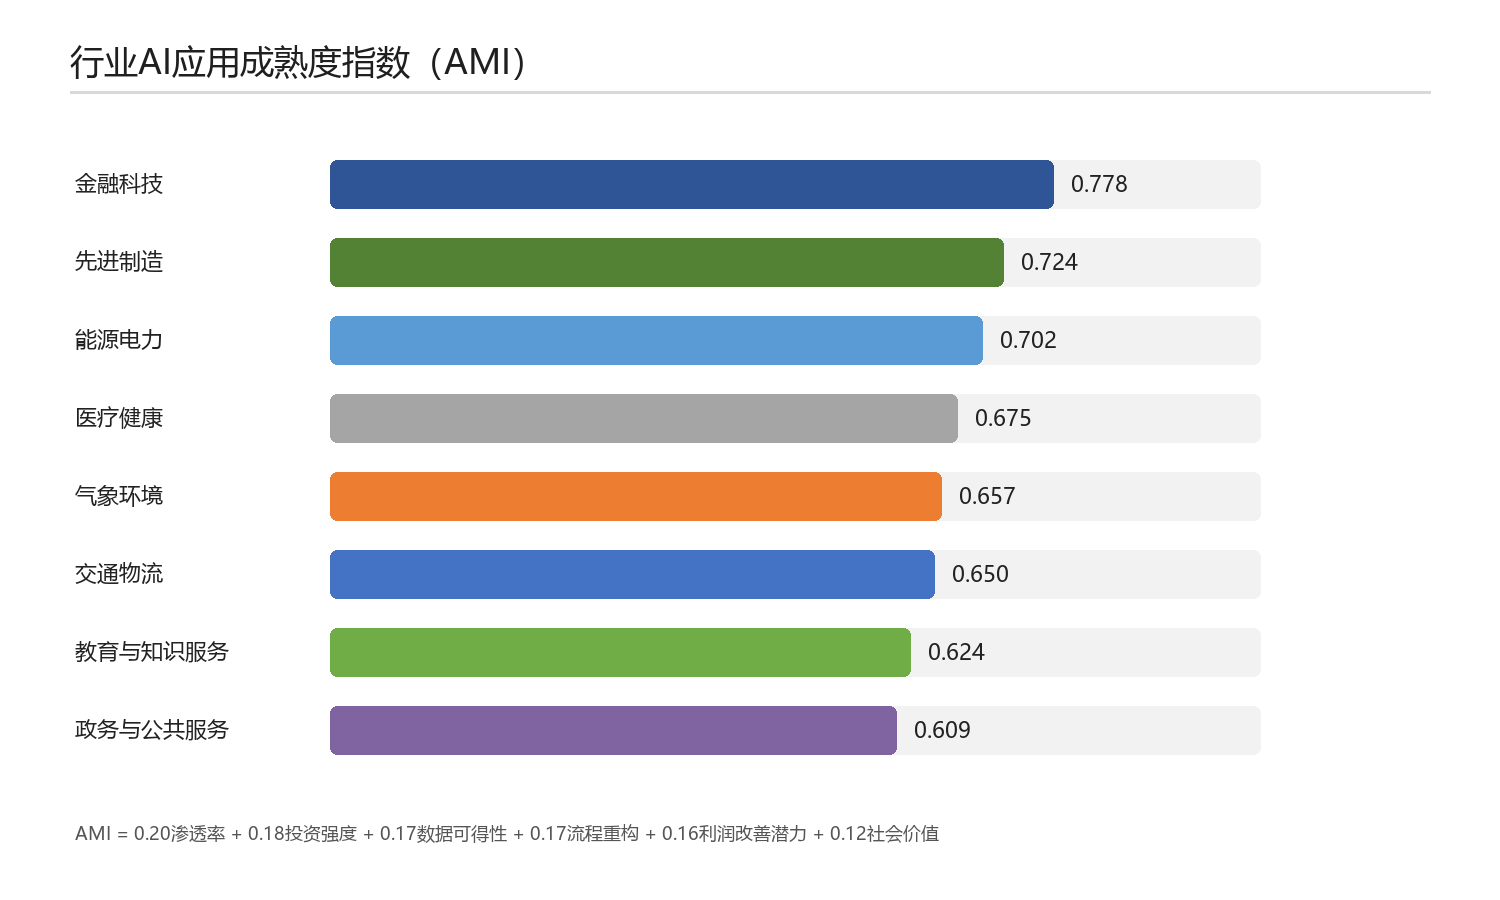
\includegraphics[width=0.95\textwidth]{charts/industry_maturity_bar.png}
\caption{行业AI应用成熟度指数排序}
\end{figure}

\begin{figure}[!htbp]
\centering
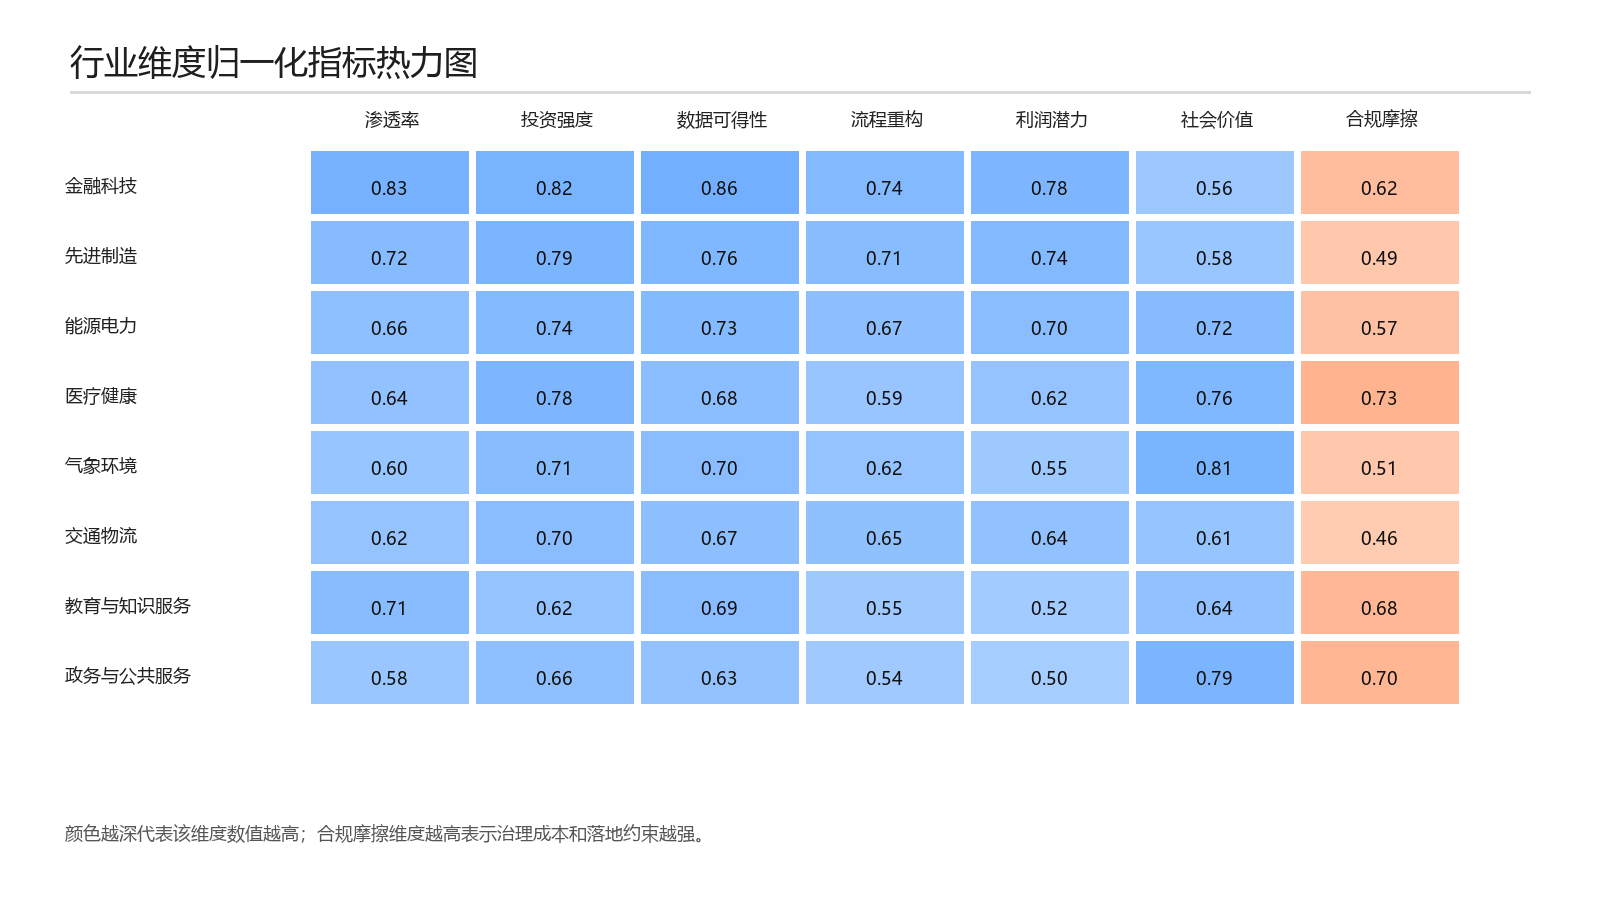
\includegraphics[width=0.98\textwidth]{charts/dimension_heatmap.png}
\caption{行业维度归一化指标热力图}
\end{figure}

\section{经济价值评估模型}
\subsection{模型框架}
AI在复杂系统中的价值形成可以分解为四个层级：数据层提供可观测性，模型层提供预测与生成能力，流程层决定模型输出能否进入真实决策，组织层决定人机协同能否稳定运行。本文据此构建图\ref{fig:framework}所示框架，将行业成熟度、价值潜力、资源约束和风险治理连接起来。

\begin{figure}[!htbp]
\centering
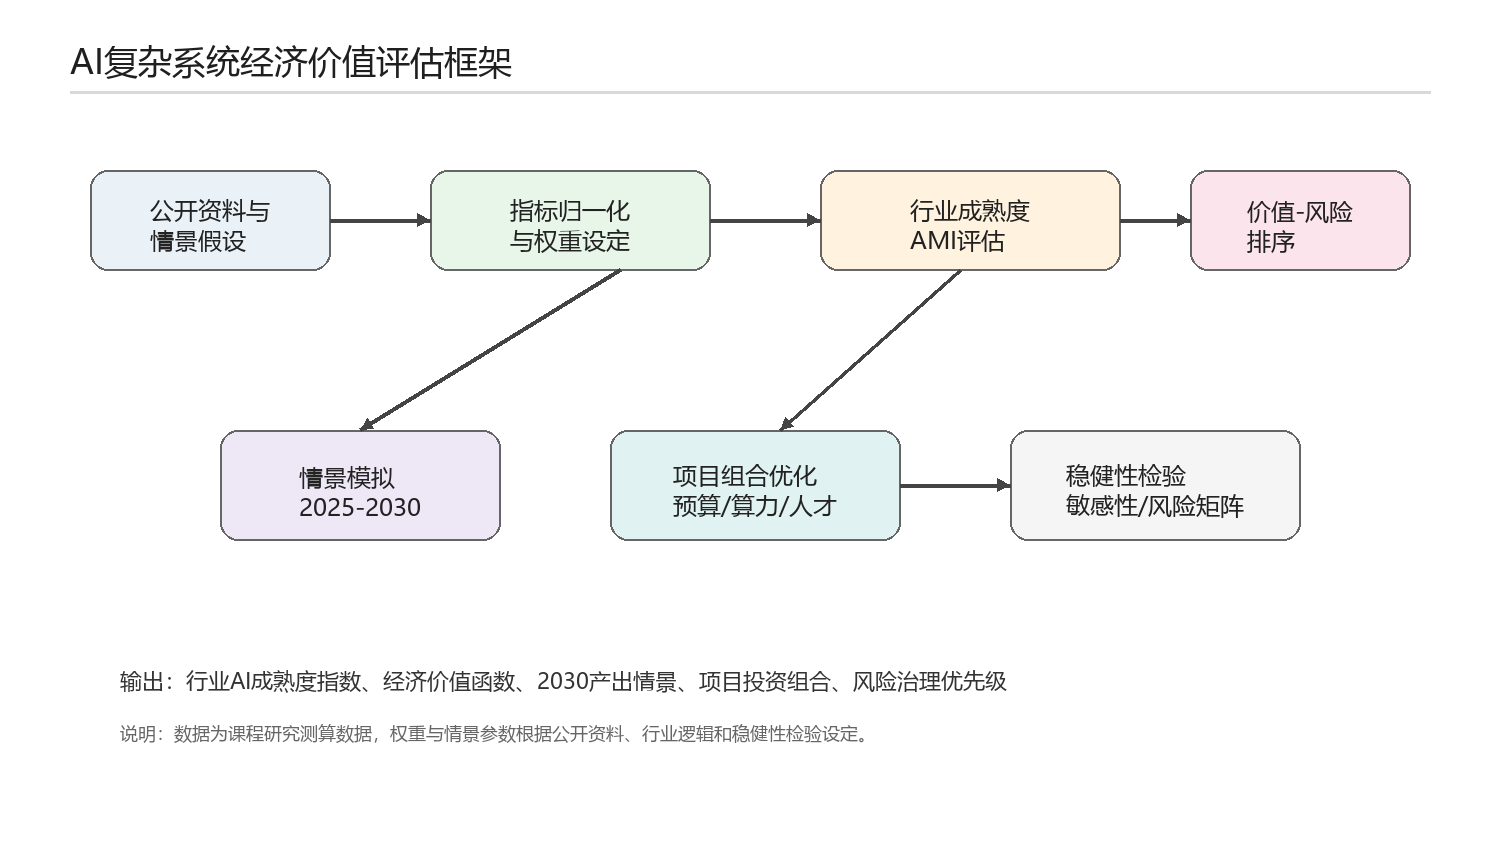
\includegraphics[width=0.98\textwidth]{charts/model_framework.png}
\caption{AI复杂系统经济价值评估框架}
\label{fig:framework}
\end{figure}

\subsection{价值潜力函数}
设行业或项目 $i$ 的经济净现值为 $NPV_i$，社会价值为 $S_i$，风险摩擦为 $R_i$，战略匹配为 $G_i$，则综合价值潜力可表示为：
\[
V_i=\alpha NPV_i+\beta S_i+\gamma G_i-\lambda R_i
\]
其中 $\alpha,\beta,\gamma,\lambda$ 反映决策者对经济收益、公共价值、战略协同和风险约束的偏好。对于商业组织，$\alpha$ 通常较高；对于公共服务系统，$\beta$ 和 $\lambda$ 应被赋予更高权重。本文在项目组合测算中采用 $V_i=NPV_i+0.6S_i$ 作为价值主项，并以风险系数作为排序和治理约束。

\subsection{成熟度-价值矩阵}
图中横轴为AMI，纵轴为价值潜力。金融科技和先进制造位于成熟度与商业价值均较高的象限，适合规模化部署；医疗健康、气象环境和政务公共服务的社会价值较高，但因合规摩擦和责任边界更强，更适合采取“高价值、强治理、分阶段”策略。

\begin{figure}[!htbp]
\centering
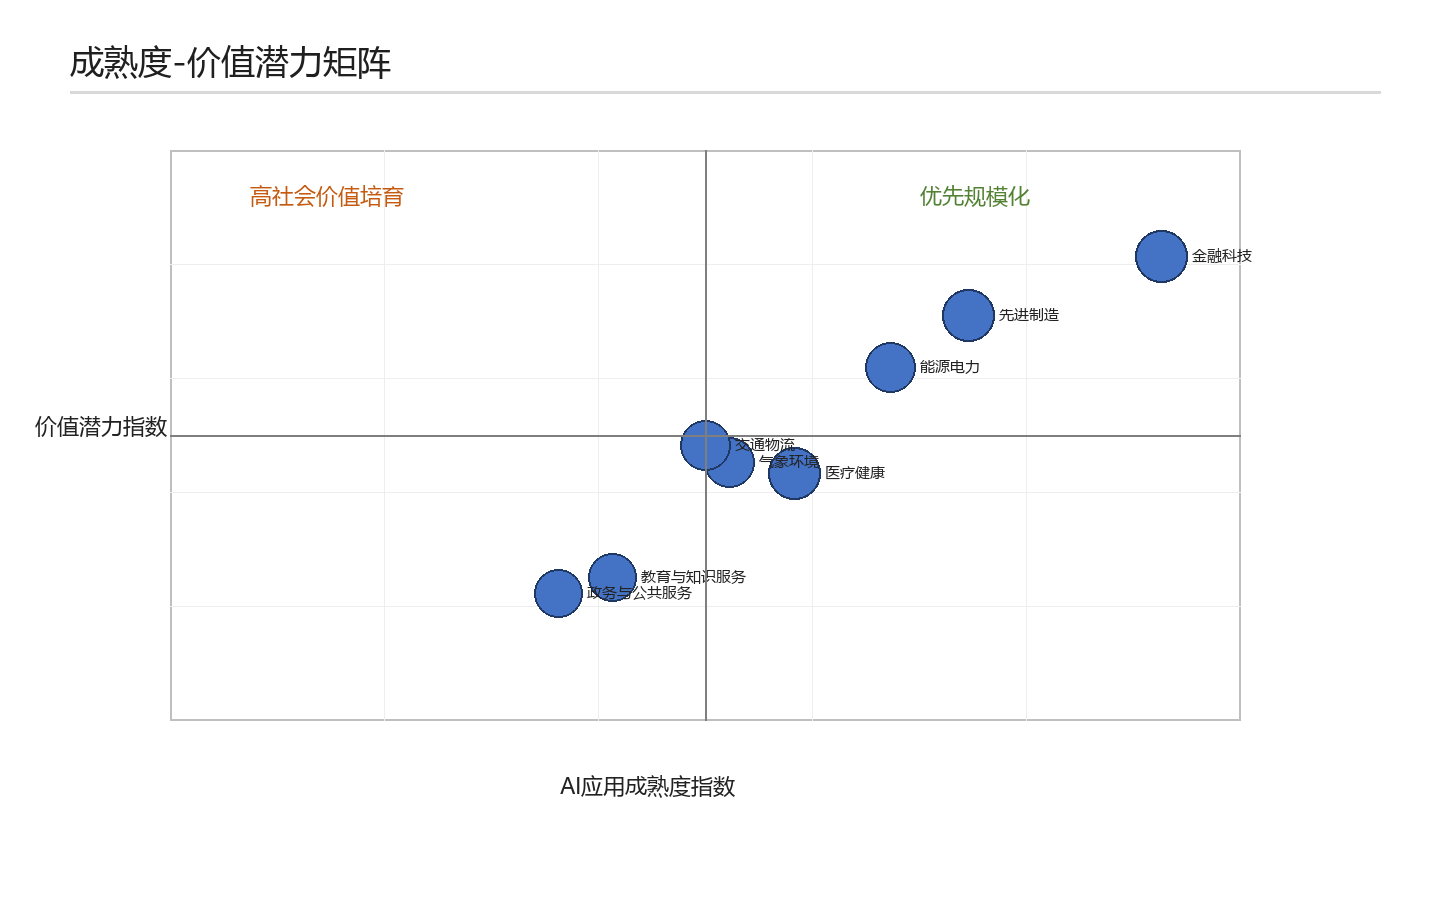
\includegraphics[width=0.92\textwidth]{charts/maturity_value_scatter.png}
\caption{成熟度-价值潜力矩阵}
\end{figure}

\section{情景模拟与结果分析}
\subsection{情景设定}
为了刻画未来不确定性，本文设置三种情景。审慎扩散情景假设AI采用受制于数据治理、合规审查和组织阻力，生产率贡献较低；基准转化情景假设行业逐步完成从试点到规模化的迁移；加速协同情景假设智能体、行业模型和流程重构形成更强互补，AI对任务结构和资本形成的影响明显增强。

\begin{table}[H]
\centering
\small
\renewcommand{\arraystretch}{1.18}
\begin{tabular}{p{0.16\textwidth} p{0.10\textwidth} p{0.14\textwidth} p{0.16\textwidth} p{0.14\textwidth} p{0.20\textwidth}}
\toprule
情景 & 年份 & 产出指数 & 生产率贡献 & 采用率 & 人机协同任务占比 \\
\midrule
审慎扩散 & 2025 & 100.0 & 0.42 & 0.45 & 0.52 \\
审慎扩散 & 2027 & 110.1 & 0.42 & 0.60 & 0.58 \\
审慎扩散 & 2030 & 126.9 & 0.42 & 0.76 & 0.64 \\
基准转化 & 2025 & 100.0 & 0.82 & 0.45 & 0.52 \\
基准转化 & 2027 & 116.2 & 0.82 & 0.70 & 0.64 \\
基准转化 & 2030 & 149.5 & 0.82 & 0.89 & 0.76 \\
加速协同 & 2025 & 100.0 & 1.28 & 0.45 & 0.52 \\
加速协同 & 2027 & 123.3 & 1.28 & 0.77 & 0.70 \\
加速协同 & 2030 & 177.6 & 1.28 & 0.94 & 0.84 \\
\bottomrule
\end{tabular}
\caption{2025--2030年AI产出情景测算}
\label{tab:scenario}
\end{table}

\begin{figure}[!htbp]
\centering
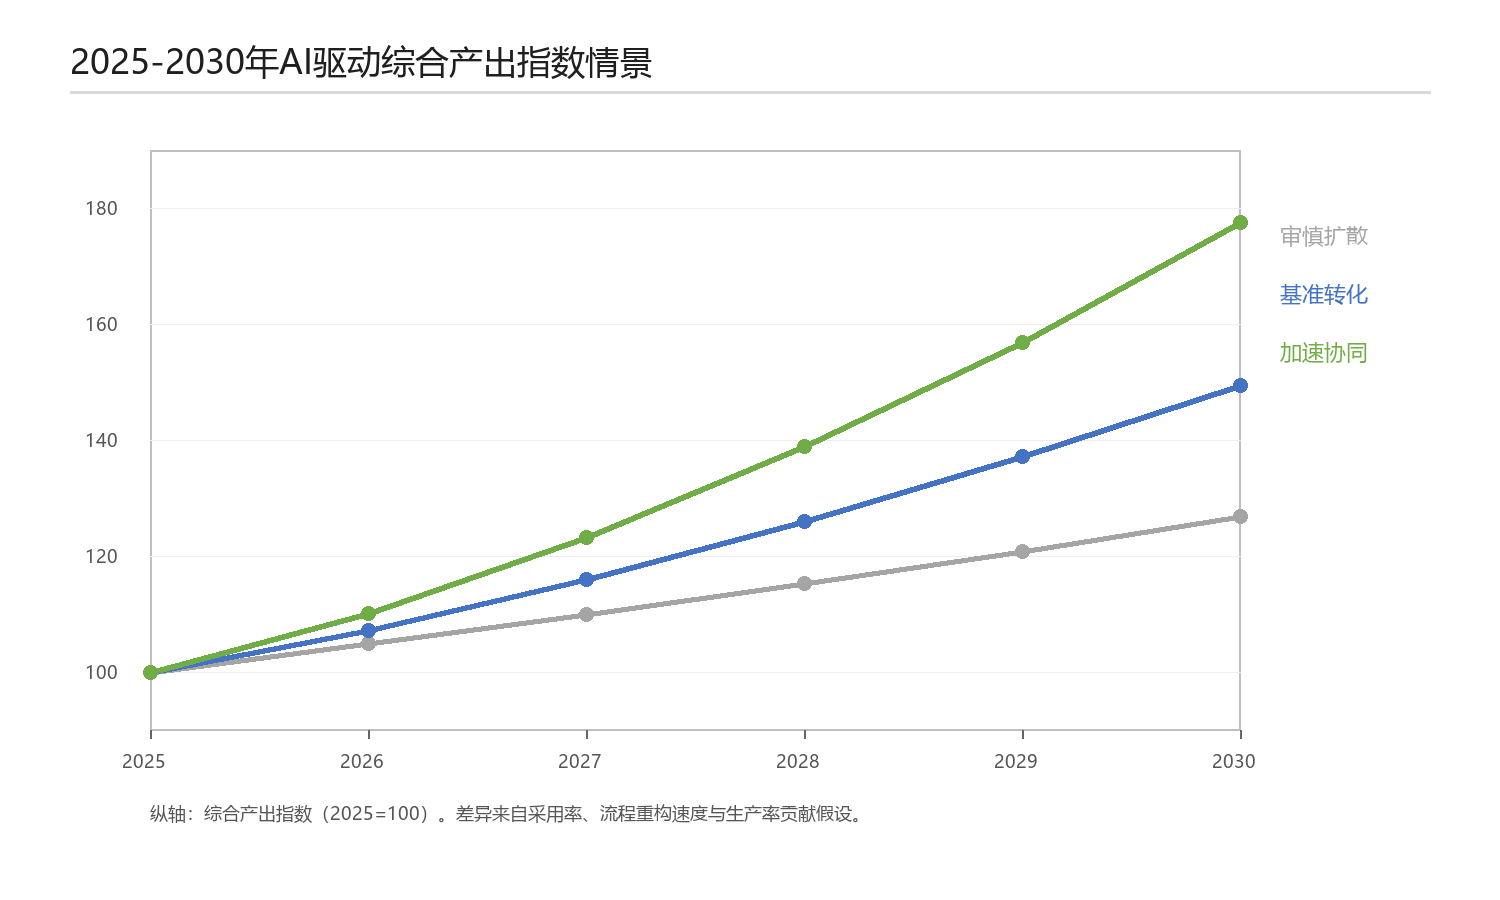
\includegraphics[width=0.92\textwidth]{charts/scenario_output_index.png}
\caption{2025--2030年AI驱动综合产出指数情景}
\end{figure}

\subsection{情景解释}
在审慎扩散情景下，2030年综合产出指数为126.9，AI更多体现为局部效率工具；在基准转化情景下，2030年指数达到149.5，说明流程重构和组织学习开始释放复合收益；在加速协同情景下，2030年指数达到177.6，但该路径对数据治理、人才供给和算力成本更敏感。由此可见，AI的长期价值并不只取决于模型能力，而取决于模型能力能否被组织结构吸收。

\section{资源优化与项目组合选择}
\subsection{优化模型}
在预算、算力和人才约束下，AI投资可以表示为0-1项目组合优化问题：
\[
\max \sum_i (NPV_i+\eta S_i)x_i
\]
\[
s.t.\quad \sum_i C_i x_i \le B,\quad \sum_i Q_i x_i \le Q,\quad \sum_i T_i x_i \le T,\quad x_i\in\{0,1\}
\]
其中 $C_i$、$Q_i$、$T_i$ 分别表示预算、算力和人才需求，$B$、$Q$、$T$ 为资源上限，$\eta$ 表示社会价值折算系数。若项目属于高风险行业，还可以加入 $R_i \le \bar R$ 或人工复核覆盖率等约束。

\begin{table}[H]
\centering
\small
\renewcommand{\arraystretch}{1.18}
\begin{tabular}{p{0.27\textwidth} p{0.14\textwidth} p{0.08\textwidth} p{0.12\textwidth} p{0.10\textwidth} p{0.08\textwidth} p{0.10\textwidth}}
\toprule
项目 & 行业 & 预算 & 经济净现值 & 社会价值 & 风险 & 价值/成本 \\
\midrule
物流路径与仓储调度优化 & 交通物流 & 14 & 46 & 16 & 0.42 & 3.97 \\
电网负荷预测与巡检智能体 & 能源电力 & 20 & 64 & 21 & 0.50 & 3.83 \\
制造视觉质检与预测维护 & 先进制造 & 18 & 58 & 18 & 0.45 & 3.82 \\
气象灾害短临预报系统 & 气象环境 & 16 & 40 & 34 & 0.49 & 3.77 \\
知识服务检索增强平台 & 教育与知识服务 & 12 & 33 & 20 & 0.53 & 3.75 \\
金融风控图谱与智能审查 & 金融科技 & 22 & 72 & 12 & 0.58 & 3.60 \\
政务服务智能问答与审批辅助 & 政务与公共服务 & 15 & 31 & 35 & 0.64 & 3.47 \\
医疗影像与临床文书助手 & 医疗健康 & 24 & 55 & 30 & 0.71 & 3.04 \\
\bottomrule
\end{tabular}
\caption{AI项目组合优化输入数据}
\label{tab:portfolio}
\end{table}

\begin{figure}[!htbp]
\centering
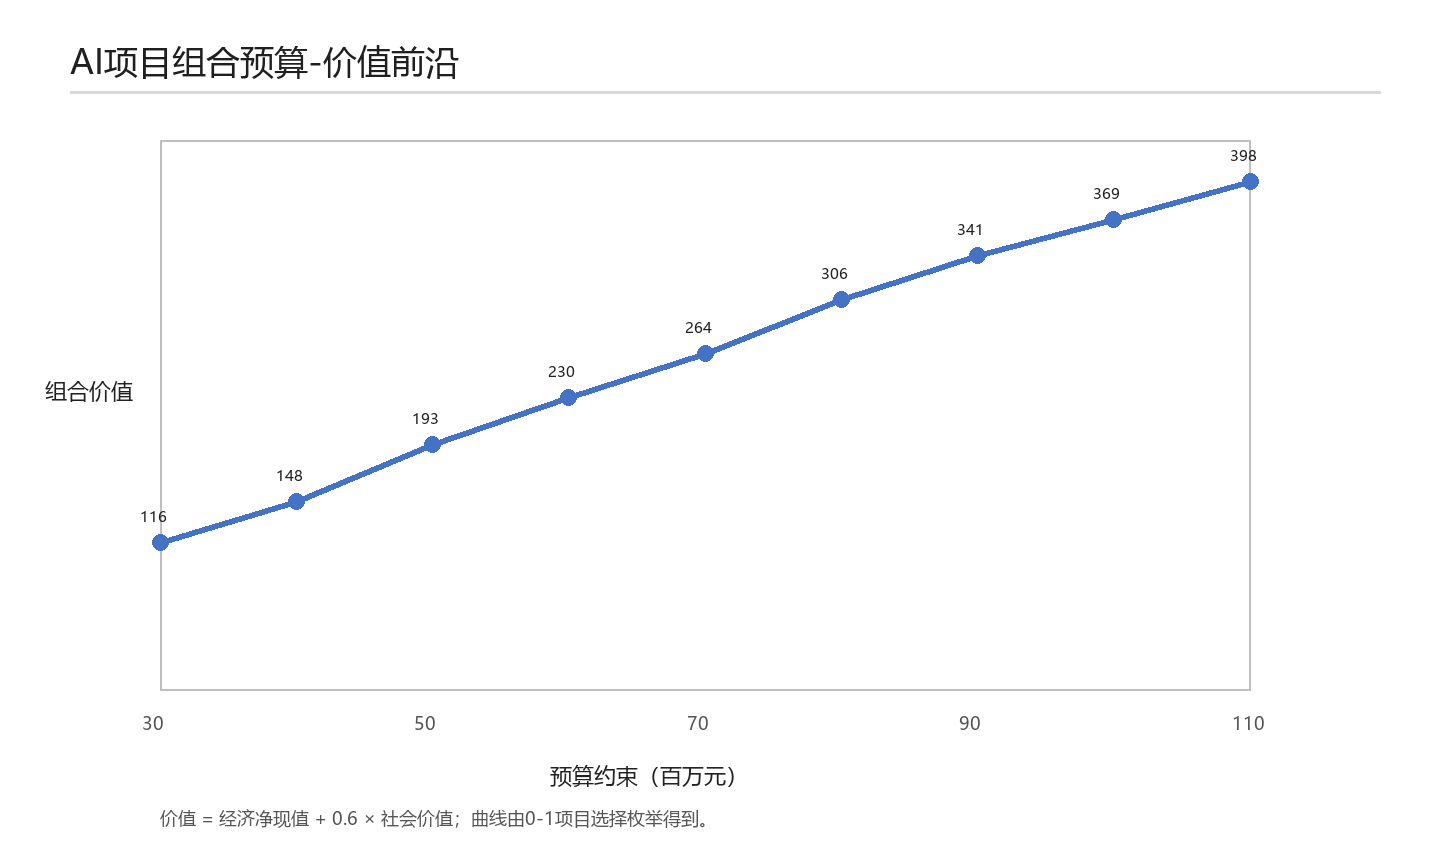
\includegraphics[width=0.90\textwidth]{charts/portfolio_frontier.png}
\caption{AI项目组合预算-价值前沿}
\end{figure}

\subsection{组合结果含义}
预算-价值前沿呈现边际收益递减特征：低预算阶段优先选择价值/成本较高、落地阻力较小的项目；预算提高后，组合开始纳入医疗、政务和气象等社会价值更高但治理成本更强的项目。因此，理性的AI投资不应只追逐单个项目ROI，而应根据组织目标在经济收益、公共价值和风险承受能力之间取得平衡。

\section{劳动力结构与风险治理}
\subsection{岗位结构影响}
AI对劳动力的影响更接近任务重组，而不是简单岗位消失。高重复、规则清晰、数字化程度高的任务更容易被自动化；需要跨情境判断、责任承担和复杂沟通的任务则更可能转向人机协同。参考WEF对AI与信息处理技术相关岗位的估计，AI相关技术同时创造和替代岗位，净影响取决于再培训速度、产业吸收能力和新岗位创造质量。

\begin{figure}[!htbp]
\centering
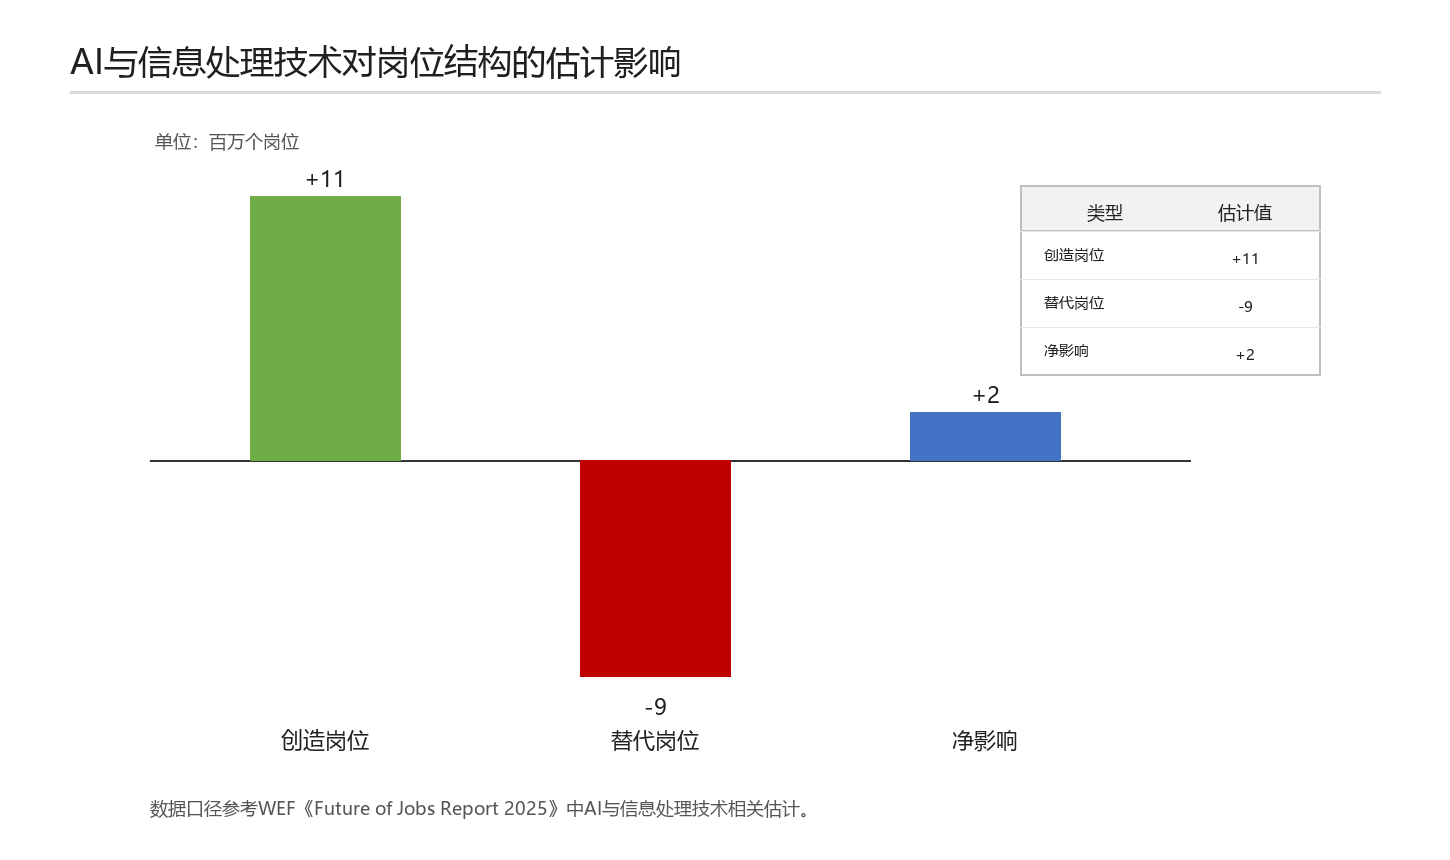
\includegraphics[width=0.78\textwidth]{charts/jobs_impact.png}
\caption{AI与信息处理技术对岗位结构的估计影响}
\end{figure}

\subsection{风险矩阵}
复杂系统中的AI风险具有联动性。模型幻觉可能引发错误决策，数据偏差可能导致分配不公，隐私泄露会触发合规责任，投资过热则可能造成收益兑现压力。本文从发生概率和影响强度两个维度构建风险矩阵，并提出治理建议。

\begin{table}[H]
\centering
\small
\renewcommand{\arraystretch}{1.18}
\begin{tabular}{p{0.07\textwidth} p{0.23\textwidth} p{0.08\textwidth} p{0.08\textwidth} p{0.46\textwidth}}
\toprule
编号 & 风险 & 概率 & 影响 & 治理建议 \\
\midrule
1 & 模型幻觉与错误决策 & 0.62 & 0.86 & 高风险场景必须保留人工复核与可追溯日志 \\
2 & 数据偏差与分配不公 & 0.58 & 0.78 & 建立数据漂移监测、样本审计和公平性指标 \\
3 & 隐私泄露与合规责任 & 0.46 & 0.90 & 采用最小化采集、脱敏、权限分层和审计 \\
4 & 投资过热与收益不达预期 & 0.55 & 0.68 & 分阶段投资，以里程碑触发扩容 \\
5 & 岗位任务重组摩擦 & 0.67 & 0.63 & 将再培训预算纳入项目可行性评价 \\
6 & 供应商锁定与技术债 & 0.42 & 0.61 & 优先开放接口、可迁移模型和多云容灾 \\
\bottomrule
\end{tabular}
\caption{AI复杂系统风险矩阵数据}
\label{tab:risk}
\end{table}

\begin{figure}[!htbp]
\centering
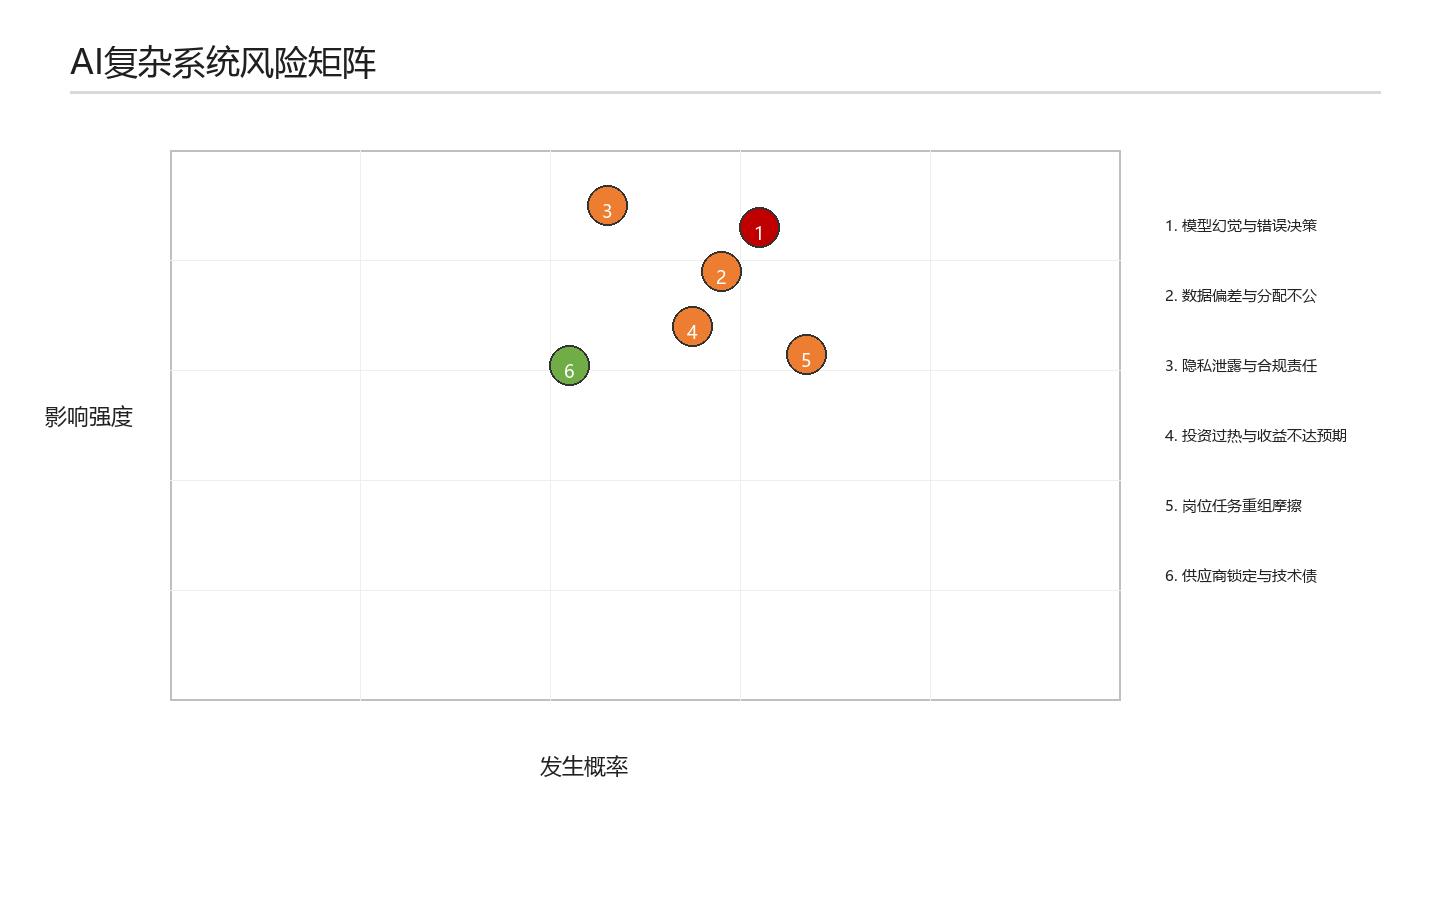
\includegraphics[width=0.88\textwidth]{charts/risk_matrix.png}
\caption{AI复杂系统风险矩阵}
\end{figure}

\section{敏感性分析与模型评价}
\subsection{敏感性分析}
本文对基准情景2030年产出指数进行单因素扰动。结果显示，采用率上限、数据质量和流程重构效率对最终结果影响最大；算力成本和合规摩擦虽也重要，但其影响更多通过项目选择和落地速度间接体现。

\begin{figure}[!htbp]
\centering
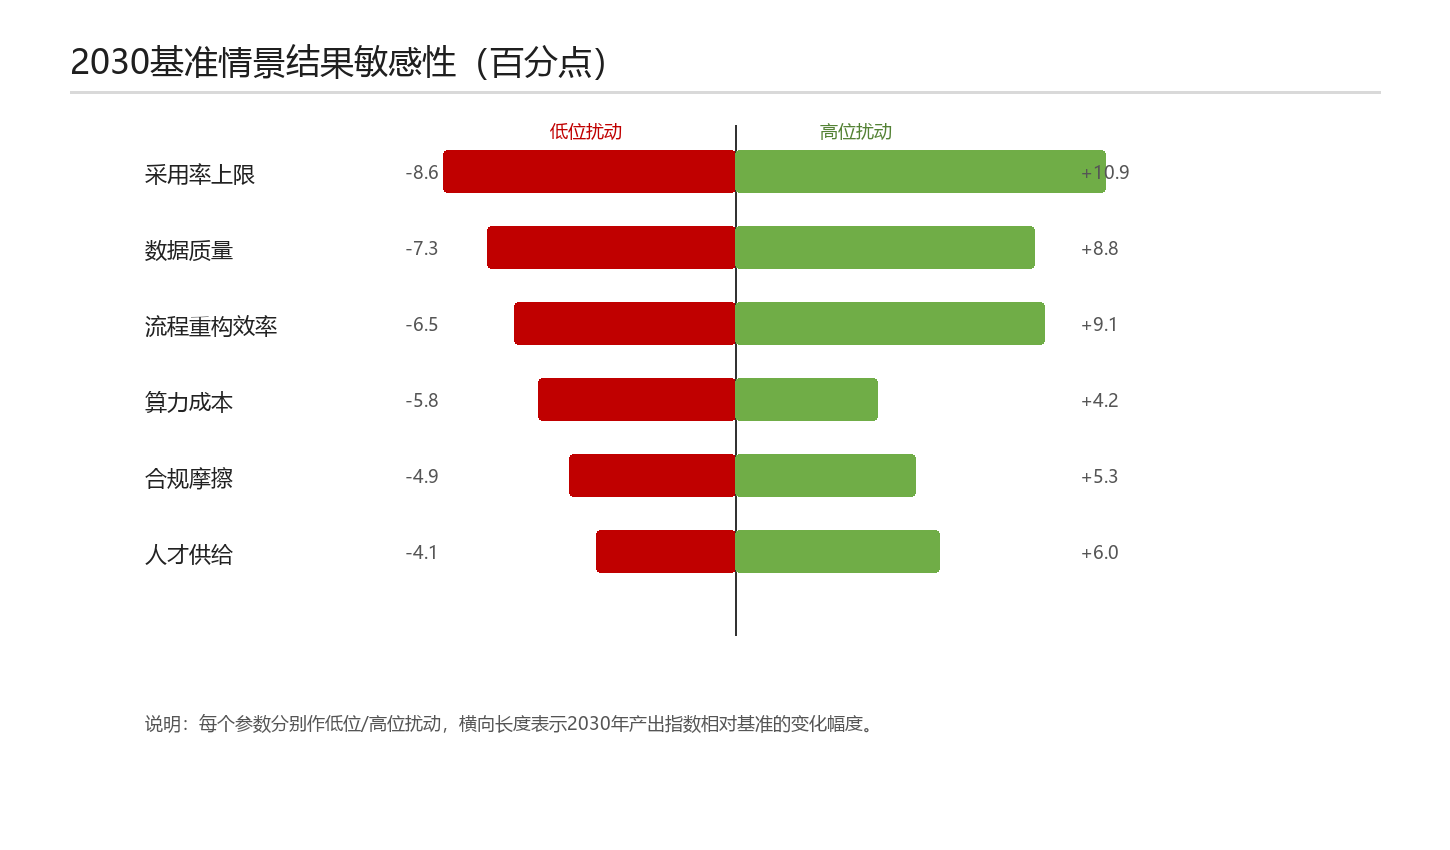
\includegraphics[width=0.90\textwidth]{charts/sensitivity_tornado.png}
\caption{2030基准情景结果敏感性分析}
\end{figure}

\subsection{模型优点}
本文模型具有三点优点。第一，指标体系可解释，能够把抽象的AI成熟度拆解为可讨论的维度；第二，价值函数兼顾经济收益和社会价值，适合复杂系统中多目标决策；第三，项目组合模型把资源约束显式化，能够解释为什么某些高价值项目不一定优先落地。

\subsection{模型局限}
模型也存在局限。首先，归一化指标依赖公开资料和研究判断，仍存在主观性；其次，行业之间的溢出效应尚未完全建模，例如能源调度优化会影响制造成本，交通物流优化会影响供应链稳定性；最后，情景模拟未引入完整随机过程，不能替代正式计量预测。后续研究可结合企业级面板数据、贝叶斯层级模型和动态系统仿真，提高估计精度。

\section{结论}
本文认为，AI在复杂系统中的经济价值不是“模型性能”的单变量函数，而是技术能力、数据基础、流程重构、人才结构和风险治理共同作用的结果。金融科技、先进制造和能源电力具备较强短期转化能力；医疗健康、气象环境和政务公共服务具有更高社会价值，但必须以强治理框架作为前提。对组织而言，AI投资应从“工具采购”转向“系统工程”：先识别高价值闭环场景，再建立数据治理和责任边界，最后通过项目组合优化实现稳健扩张。对政策制定者而言，推动AI应用的关键不是单纯扩大模型供给，而是降低高质量数据、算力、人才和合规基础设施的协同成本。

\clearpage
\begin{thebibliography}{99}
\bibitem{S1} Stanford HAI. \textit{AI Index Report 2025}.
\bibitem{S2} McKinsey. \textit{The State of AI in 2025}.
\bibitem{S3} World Economic Forum. \textit{Future of Jobs Report 2025}.
\bibitem{S4} OECD.AI. \textit{Macroeconomic productivity gains from artificial intelligence in G7 economies}.
\bibitem{S5} 国务院. 《关于深入实施“人工智能+”行动的意见》.
\bibitem{S6} 工业和信息化部. 人工智能产业公开信息.
\end{thebibliography}

\end{document}
